%!tex root=./thesis.tex
\chapter{Extended Radio Sources and Astroinformatics}
\label{cha:background}

I'll need to explain the purpose of this chapter and give a brief outline. There'll be three sections, and I'll briefly summarise them here.

    \begin{figure}[ht]
        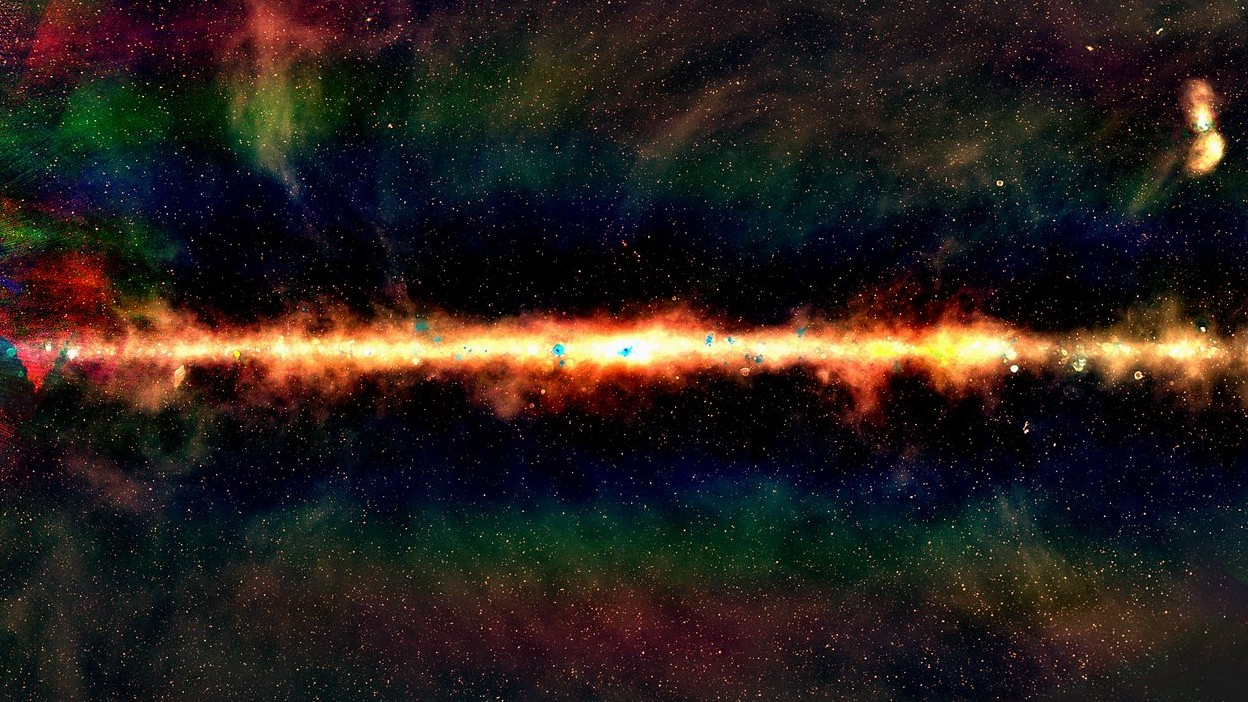
\includegraphics[width=\textwidth]{images/gleam.jpg}
        \caption[False-colour image of the radio sky from the GLEAM survey.]{\label{fig:gleam} False-colour image of the radio sky from the GLEAM survey. (Image: Natasha Hurley-Walker, Curtin University/ICRAR \citeneeded)}
    \end{figure}

\section{The Extragalactic Radio Sky}
\label{sec:extragalactic-radio-sky}

    The extragalactic sky appears quite different at different wavelengths. While an optical observer may look at a distant galaxy and see spirals and halos, an infrared observer will see discs and dust. What does the radio astronomer see? 
    \autoref{fig:gleam} shows a false-colour image of the radio sky. The plane of the Milky Way is clearly visible through the centre, but nearly every other object in this image is a galaxy. These galaxies fall into two main categories: those that emit radio due to star formation (called \defn{star-forming galaxies}), and those that emit radio due to \defn{active galactic nuclei} (AGN).

    Non-AGN emission from distant galaxies traces the recent star-formation rate (SFR). Besides low-power thermal emission, stellar radio emission from galaxies mainly comes from massive ($\gtrapprox 8$ M$_\odot$) stars, through two emission mechanisms. The first is through H~II regions, which are ionised by such stars. The ionised electrons emit bremsstrahlung radiation at radio wavelengths. The second emission mechanism is supernovae. Massive stars may end their lives in Type II and Type Ib supernova, which can result in supernova remnants. These remnants emit synchrotron radiation. Massive stars like these are short-lived ($\lessapprox 3 \times 10^7$ yr), and the corresponding emitting electrons have similarly short lifetimes ($\lessapprox 10^8$ yr). The radio effects of these stars are therefore also short-lived, which is why radio emission traces the recent SFR \citep{condon_radio_1992}. Star formation-associated emission is mainly found in the disc of spiral galaxies, as this is where the star formation rate is highest. In particular, there is no star-forming radio emission extending outside of the galaxy proper. The radio power emitted by these galaxies at 1.4~GHz is on the order of $10^{18}$--$10^{23}$~W~Hz$^{-1}$ \citep{condon_radio_1992}. For a radio survey like the NVSS, with a detection limit of 2.3~mJy, this luminosity range corresponds to a maximum redshift range of $0.0004$--$0.1272$. Upcoming surveys such as EMU, with 5$\sigma$ detection thresholds of 50~$\upmu${}Jy \citep{norris_emu_2011}, will push this range to $0.0030$--$0.6684$.

    AGN are energetic objects at the centre of galaxies, powered by supermassive black holes. They emit synchrotron radiation from accelerating relativistic electrons in strongly-magnetised plasma. The radio luminosity of AGN ranges from $10^{22}$--$10^{30}$ W~Hz$^{-1}$\citeneeded at 1.4~GHz, making them some of the most luminous objects in the universe \citeneeded. They are therefore visible throughout the universe, with the most distant AGN detected at a redshift of 7 \citeneeded. Depending on the orientation and type of AGN, the radio emission may be very extended outside of the galaxy itself---up to megaparsec scales---and this emission may have complex structure. Perhaps the most impressive local example is Centaurus A (Cen A), the prominent double-lobed cloud in the upper-right of \autoref{fig:gleam} extending over 8 degrees across the sky. \autoref{sec:agn} discusses AGN in more detail.

    Most AGN are compact and unresolved in any given radio survey due to the distance at which they can be detected and their orientation or type. This means that their structure does not always help distinguish AGN radio emission from star-forming radio emission. How can we tell these apart? Synchrotron emission has a considerably steeper spectral index than bremsstrahlung, but synchrotron emission dominates the bremsstrahlung in star-forming galaxies \citep{condon_radio_1992}. Some division can be made with access to optical spectral information about the host galaxy of the radio emission \citep[e.g.][]{mauch_radio_2007, groves_distinguishing_2008}, but radio emission is detectable at much greater distances than good quality optical spectra can be obtained at, making this solution impractical for many galaxies. \todo{so how do we do it then?}

    From the size scales described above, it should be clear that a survey of extended radio sources will be dominated by AGN. Nevertheless, star-forming galaxies present a significant part of the radio population, and the fraction of the radio sky they comprise varies significantly with survey parameters.

    % \item the extra-galactic radio sky (gotta start here to be interesting?): \begin{itemize}
    %     \item star-forming galaxies
    %     \item AGN
    %     \item the galactic plane and foreground
    % \end{itemize}

    % The last major component of the radio sky is the galactic plane of the Milky Way.

    % \begin{itemize}
    %     \item how often do we expect to see AGN vs star formation?
    %     \item how is this affected by observational parameters?
    %     \item how do we tell the difference?
    %     \item extended sources are mainly AGN in the surveys we care about
    %     \item what gets in our way of seeing extragalactic stuff?
    % \end{itemize}

\section{Radio emission}
\label{sec:radio-astronomy}

    Electromagnetic radiation in radio frequencies---about 10~MHz--1~THz \citep{condon_essential_2016}---is called \defn{radio emission}. This is a very broad range of frequencies and so radio astronomy covers a very broad range of astrophysical phenomena, from cosmological background radiation to neutron stars. The focus of this thesis is the exciting, dynamic, and so-called `violent universe' of radio galaxies. These galaxies are observed through their emission of synchrotron radiation and are studied through their observed physical structure, the intensity and spectroscopic properties of their radiation, and the polarisation and spectropolarimetric properties that are uniquely visible in radio. This section introduces synchrotron radiation and radio polarisation.

    \subsection{Synchrotron radiation}
    \label{sec:synchrotron}

        Most radio emission from AGN is \defn{synchrotron radiation}, produced by relativistic charged particles accelerating in a magnetic field. A non-relativistic charged particle will spiral with a fixed angular frequency when it moves in a magnetic field in a process called \defn{gyro radiation}. Synchrotron radiation is a relativistic effect: it can be thought of as gyro radiation Lorentz transformed to energies much greater than $mc^2$. The spectrum of synchrotron radiation follows a power law \citep{condon_essential_2016}:
        \begin{equation}
            \label{eq:spectral-index}
            S(\nu) \propto \nu^{\alpha}.
        \end{equation}
        $\alpha$ is called the \defn{spectral index}\footnote{Note that the sign of $\alpha$ varies by convention, and both $S \propto \nu^{\alpha}$ and $S \propto \nu^{-\alpha}$ exist in the literature.}. It is related to the energy distribution of the emitting electrons: assuming that the electron energy distribution follows a power law (which it generally does\citeneeded), where the number density of electrons at a given energy $E$ is given by
        \begin{equation}
            n(E) \propto E^\Gamma,
        \end{equation}
        then
        \begin{equation}
            \alpha = \frac{\Gamma - 1}{2}.
        \end{equation}
        The spectral index for astronomical objects tends to range from -2 to 2\citeneeded.


    \subsection{Polarisation}
    \label{sec:polarisation}

        Electromagnetic radiation consists of waves of self-propagating, orthogonal electric and magnetic fields. The orthogonality of these two waves allows us to characterise the radiation just by the electric field. As a transverse wave, the electric field travels at an angle. This angle and its behaviour is called the \defn{polarisation} of the wave.

        The polarisation can be characterised by decomposing the electric field into orthogonal components $E_x$ and $E_y$, letting $\hat z$ denote the axis of propagation:
        \begin{equation}
            \vec E = (\hat x E_x \exp(i \varphi_x) + \hat y E_y \exp(i \varphi_y)) \exp(i (\vec k \cdot \hat z - \omega t)).
        \end{equation}
        In an astronomical context, $\hat z$ is the line-of-sight from the source of the radiation to the observer. $\vec k$ is the \defn{wave vector} which points in the direction of travel and has magnitude $2\pi/\lambda$ and $\omega = 2\pi\nu$ is the \defn{angular frequency}. $\varphi_x$ and $\varphi_y$ are the phase offsets of each component. As this wave propagates along the line-of-sight toward an observer, the electric field oscillates in an ellipse across the $x$--$y$ plane. When the two components are in phase, this ellipse is degenerate and the radiation is called \defn{linearly polarised}. When the two components are perfectly out of phase, the ellipse is a circle, and the radiation is called \defn{circularly polarised}. Of course, any ellipse in between these extremes is also possible. For this reason, we decompose the polarisation into linearly polarised components and a circularly polarised component, called \defn{Stokes parameters}. These are \citep{condon_essential_2016}:
        \begin{align}
            \label{eq:stokes-i}
            I &= \frac{1}{R_0} \mathbb E_t[E_x^2 + E_y^2],\\
            \label{eq:stokes-q}
            Q &= \frac{1}{R_0} \mathbb E_t[E_x^2 - E_y^2],\\
            \label{eq:stokes-u}
            U &= \frac{1}{R_0} \mathbb E_t[2 E_x^2 E_y^2 \cos (\varphi_x - \varphi_y)],\\
            \label{eq:stokes-v}
            V &= \frac{1}{R_0} \mathbb E_t[2 E_x^2 E_y^2 \sin (\varphi_x - \varphi_y)].
        \end{align}
        $I$ is the \defn{total intensity}. $Q$ and $U$ together describe the linear polarisation and together can be used to define the \defn{polarisation angle} $\chi$:
        \begin{equation}
            \label{eq:polarisation-angle}
            \tan (2 \chi) = \frac{U}{Q}.
        \end{equation}
        $V$ is the circular polarisation and describes the eccentricity of the ellipse. For most extragalactic sources, the circular polarisation is zero \citeneeded because \todo{reasons}. Incoherent radiation may be composed of radiation with many different polarisations, and these polarisations may fully or partially cancel out: this is called \defn{unpolarised} or \defn{partially-polarised} respectively. The total intensity of polarised radiation is called the \defn{polarised intensity} and is given by
        \begin{equation}
            \label{eq:polarised-intensity}
            P^2 = Q^2 + U^2 + V^2.
        \end{equation}
        Note that $P^2 \leq I^2$. The \defn{fractional polarisation} is the ratio between these two intensities:
        \begin{equation}
            p = \frac{P}{I}.
        \end{equation}

        The synchrotron radiation from AGN is polarised, though this polarisation is not always detectable \citeneeded \todo{forward reference to AGN?}. Additionally, the most common non-AGN cause for radio emission is star-formation, which does not have detectable polarisation. Polarisation is therefore an excellent way to confirm that a radio source is an AGN.

        Polarisation can also be used to describe the magnetic structure of both AGN and intervening medium. As polarised light from distant galaxies makes its way to us, magnetised plasma along the way can cause the polarisation angle to rotate due to the Faraday effect. The amount of rotation is called the \defn{Faraday depth} $\phi$, and is related to the electron density $n_e$ and the line-of-sight magnetic field strength $\vec B \cdot \hat{z}$ of the intervening medium:
        \begin{equation}
            \label{eq:faraday-depth}
            \phi(x, y) = \frac{e^3}{8\pi^2\epsilon_0m_e^2c^3} \int_{\mathrm{there}}^{\mathrm{here}} n_e(x, y, z) \vec B(x, y, z) \cdot \mathrm{d}\hat{z}\ \mathrm{rad}\ \mathrm{m}^{-2}.
        \end{equation}
        Here $\mathrm{d}\vec r$ is the infinitesimal path length in pc \citep{brentjens_faraday_2005} \todo{Check the units on this, and maybe get the actual form for 0.81.}. Within the synthesised beam of a radio telescope\todo{forward reference to beams}, multiple Faraday depths may exist. If the polarised spectrum of the source is observed at multiple frequencies, then these multiple depths can be disentangled even though they spatially overlap in the radio image. This can provide insight into the polarised structure of the source as well as the intervening medium. The leading constant is around $2.62 \times 10^{-13}$~T$^{-1}$, more commonly written as 0.812 pc $\upmu$G$^{-1}$ cm$^{-1}$ in CGS units with $B$ in $\upmu$G and $z$ in pc.

        If the entire beam has precisely one Faraday depth $\phi$, then the polarised structure is called a \defn{Faraday screen}. In this degenerate case, the relationship between the polarisation angle $\chi$ and the squared wavelength $\lambda^2$ is linear:
        \begin{equation}
            \chi = \chi_0 + \phi \lambda^2.
        \end{equation}
        $\phi$ is then called the \defn{rotation measure}. Until very recently, the frequency resolution of polarised surveys was insufficient to meaningfully separate most complex arrangements of Faraday depths, and so most sources were characterised entirely in terms of their rotation measure \citep[e.g.][]{taylor_rotation_2009}. Advancing telescope technology and emphasis on polarisation science has opened new frontiers in spectropolarimetry and upcoming and ongoing surveys (e.g. RACS and POSSUM) will likely produce Faraday depth catalogues instead of rotation measures. Of course, no physical source has a precise Faraday depth, as there is always intrinsic scatter. Along the line of sight, if we assume Gaussian noise in an otherwise-constant $n_e$ i.e. $n_e(z) \sim \mathcal N(\overline n_e, \sigma_{n_e}^2)$, and a constant $B$ for simplicity, then we find
        \begin{equation}
            \phi \sim \mathcal N\left(\frac{e^3}{8\pi^2\epsilon_0m_e^2c^3} B \overline n_e, \frac{e^3}{8\pi^2\epsilon_0m_e^2c^3} B \sigma_{n_e}^2\right),
        \end{equation}
        that is, the depth has an uncertainty proportional to the magnetic field strength and the noise in $n_e$. A similar result follows for noise in $B$ only. There is no analytic solution for noise in both $B$ and $n_e$, but if we approximate the integrand as a Gaussian by calculating the mean and variance we find
        \begin{equation}
            \phi \sim \mathcal N\left(\frac{e^3}{8\pi^2\epsilon_0m_e^2c^3} \frac{\overline n_e \sigma_B^2 + \overline B \sigma_{n_e}^2}{\sigma_B^2 + \sigma_{n_e}^2}, \frac{e^3}{8\pi^2\epsilon_0m_e^2c^3} \frac{\sigma_{n_e}^2 \sigma_B^2}{\sigma_{n_e}^2 + \sigma_B^2}\right).
        \end{equation}
        We observe multiple lines-of-sight that are coalesced into one within the beam. Due to this noise, even with constant $n_e$ and $B$ across a source, we can see multiple Faraday depths as each line-of-sight is a sample from the above distribution.

        %     \label{eq:faraday-depth-intrinsic-dispersion-simple}
        %     \phi(x, y) \sim \mathcal N\left(10^{-16} \times 0.81 \frac{D}{1\ \mathrm{pc}} \overline n_e \overline B_{\perp}, 10^{-16} \times 0.81 \frac{D}{1\ \mathrm{pc}} \sigma_{n_e}\right).
        % \end{equation}

        \todo{Need a bit on Faraday screens, Faraday complexity?}

\section{Active Galactic Nuclei}
\label{sec:agn}
    % \begin{itemize}
    %     \item AGN: \begin{itemize}
    %         \item jets
    %         \item lobes
    %         \item the unified model
    %         \item classes including FRI and FRII, radio loud and radio quiet... etc
    %         \item polarisation structure
    %         \item spectral index
    %         \item environmental interaction with jets and lobes, including how much power they inject according to simulations and literature
    %         \item host galaxies
    %     \end{itemize}
    %     \item AGN throughout the universe: \begin{itemize}
    %         \item expected RLF/distribution
    %         \item getting brighter back in time
    %         \item FRI/FRII? radio loud, radio quiet?
    %         \item how many AGN are there?
    %         \item how do AGN tie into galaxy evolution and feedback?
    %     \end{itemize}
    % \end{itemize}

    AGN are some of the most energetic objects in the Universe. They both provide a laboratory for extreme physics and are a key part of the life cycle of a galaxy \citep{heckman_coevolution_2014}. Powered by a supermassive black hole, they convert gravitational potential energy into intense electromagnetic radiation at a broad range of frequencies. AGN that produce strong radio emission are called radio AGN, and methods of observing the complex structures that these radio AGN form are the focus of this thesis.

    \subsection{The unified model}
    \label{sec:unified-model}

        \begin{figure}
            \centering
            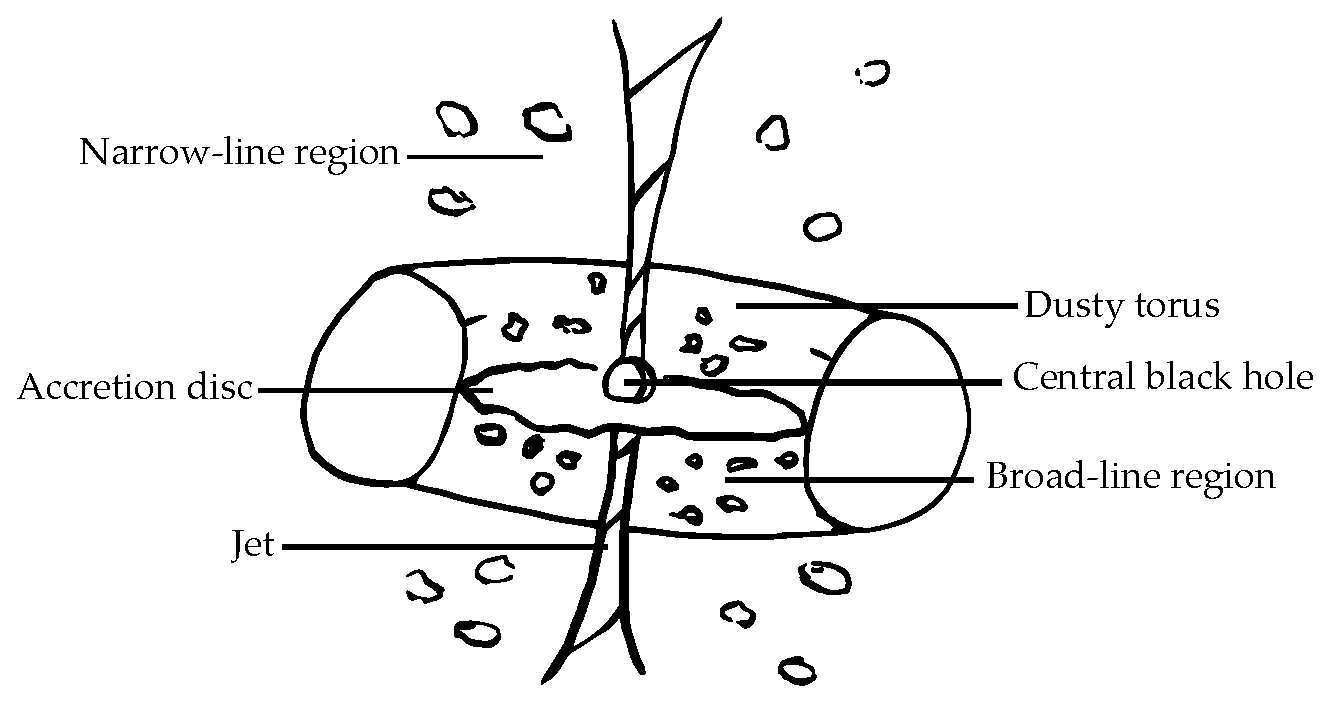
\includegraphics[width=\textwidth]{images/agn.eps}
            \caption{\label{fig:agn} The unified model of AGN.}
        \end{figure}

        \begin{figure}
            \centering
            \begin{subfigure}{0.45\textwidth}
                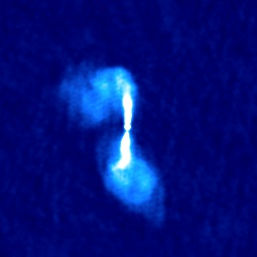
\includegraphics[width=\textwidth]{images/3C_272.1.jpg}
                \caption{M84/3C 272.1}
                \label{fig:m84}
            \end{subfigure}
            \begin{subfigure}{0.45\textwidth}
                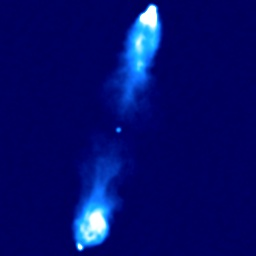
\includegraphics[width=\textwidth]{images/3C_223.jpg}
                \caption{3C 223}
                \label{fig:3C223}
            \end{subfigure}
            \caption[Examples of a FRI and a FRII radio galaxy.]{\label{fig:fri-frii} Examples of (a) a FRI \citep{laing_rotation_1987} and (b) a FRII radio galaxy \citep{leahy_vla_1991}. Both are shown with an arcsinh stretch and were observed with the VLA.}
        \end{figure}

        At their core, AGN are an accreting \defn{supermassive black hole}: a body so dense that even light cannot escape its gravitational pull, with mass on the order of $10^7$--$10^9\ \mathrm{M}_\odot$ \citeneeded{}. Such black holes seem to exist at the centre of galaxies\citeneeded{} and these galaxies are called \defn{host galaxies}. The current understanding of the structure of an AGN is as follows \citep{urry_unified_1995}. The black hole is surrounded by an accretion disc emitting in ultraviolet and X-ray. Beyond this is the broad-line region, named for the Doppler-broadened emission lines emitted by the energetic clouds of material surrounding the accretion disc. The broad-line region and accretion disc are themselves surrounded by a dusty torus (or some other disc-like structure) which prevents light from the centre of the AGN being observed from the sides. Further still from the accretion disc is the narrow-line region, where lower-energy gas produces narrow emission lines. From either side of the disc, an AGN produces two collimated outflows of relativistic plasma called {jets}, and these jets interact with gas in the host galaxy to produce bright radio emission. As the jets disperse further out from the centre of the AGN they widen into plumes of plasma known as \defn{lobes}. This model of AGN unifies different observed classes of AGN by their orientation and luminosity, and is hence known as the \defn{unified model} \citep{antonucci_unified_1993}.

        There are many different ways to divide the set of radio AGN into classes. By morphology, radio AGN are often divided by the structure of the jets and lobes: Fanaroff-Riley type I (FRI) and Fanaroff-Riley type II (FRII) are the most striking examples, with FRI having wavy, diffuse lobes; and FRII having long, tightly-collimated jets and sharp-edged lobes with bright hot-spots \citep{urry_unified_1995}. FRII are also generally higher-luminosity \citep{fanaroff_morphology_1974} than FRI and therefore make up the majority of observed extended radio sources throughout the Universe. AGN can also be divided into \defn{radiative-mode} and \defn{jet-mode} by how they expel their energy \citep{heckman_coevolution_2014}. Radiative-mode AGN produce radiative energy in amounts higher than 1 percent of their Eddington limit, while jet-mode AGN mainly output energy through their jets. The Eddington limit describes the maximum luminosity that a compact object can emit, and is given in \autoref{eq:eddington} \citep{rybicki_radiative_1979}:
        \begin{equation}
            L_{\mathrm{Eddington}}(M) = \frac{4\pi G M m_p c}{\sigma_T}.
            \label{eq:eddington}
        \end{equation}
        Optical emission observed near the centre of the AGN can be used to divide radio AGN into broad-line and narrow-line galaxies: the former are AGN seen end-on, and the latter are AGN seen edge-on with the dusty torus obscuring the broad-line region. These narrow-line galaxies are usually the only ones for which we see significant extended structure.

    \subsection{Extended structure}
    \label{sec:extended-structure-of-agn}

        The jets and lobes of AGN can be very extended, with the largest known radio galaxies measuring over 4 Mpc end-to-end \citep{machalski_understanding_2011}. This is much larger than the radius of their host galaxies, and so the jets and lobes of AGN are uniquely posed to interact with the local environment. Environmental interactions both within and outside the host galaxy warp and distort the jets and lobes. Within the galaxy, \todo{something about internal pressures? simulations??}. Outside the galaxy, the jets and lobes are bent by the intra-cluster medium and neighbouring galaxies \citep[ICM;][]{garon_radio_2019, rodman_radio_2019} and this structure may even be used as a probe for cluster environments \citep{banfield_radio_2016}.

        \begin{figure}
            \centering
            \begin{subfigure}{0.3\textwidth}
                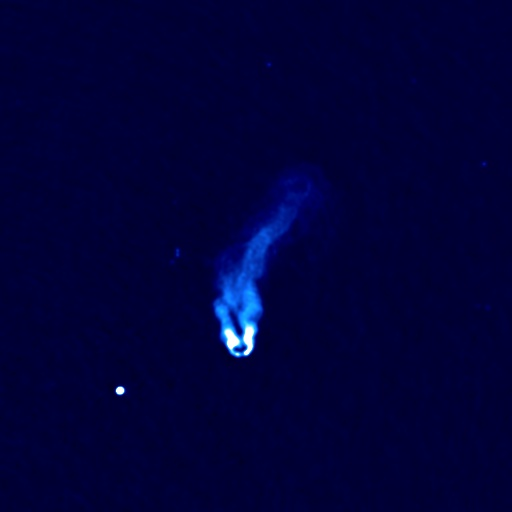
\includegraphics[width=\textwidth]{images/3C_83.1B.jpg}
                \caption{3C 83.1B}
                \label{fig:3C83-1B}
            \end{subfigure}
            \begin{subfigure}{0.3\textwidth}
                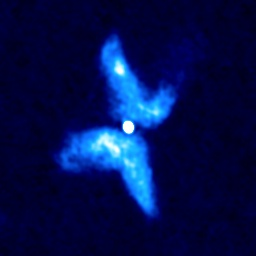
\includegraphics[width=\textwidth]{images/3C_315.jpg}
                \caption{3C 315}
                \label{fig:3C315}
            \end{subfigure}
            \begin{subfigure}{0.3\textwidth}
                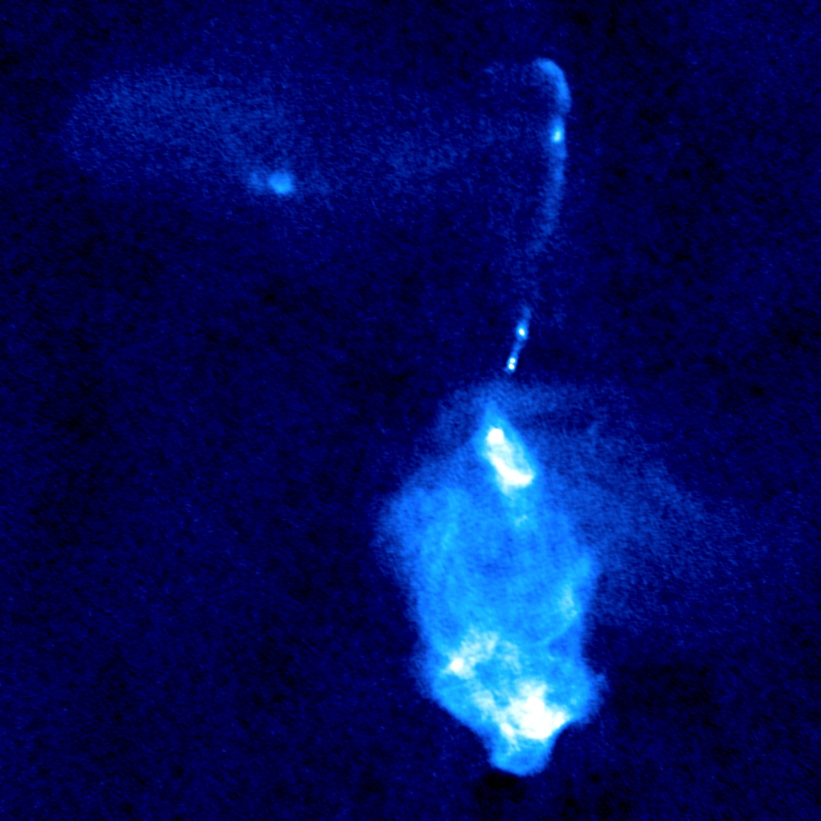
\includegraphics[width=\textwidth]{images/3C_433.jpg}
                \caption{3C 433}
                \label{fig:3C433}
            \end{subfigure}
            \caption[Three radio galaxies with interesting structure.]{Radio galaxies, displayed with an arcsinh colour scale. All images were taken with the VLA. (a) is a narrow-angled tail radio galaxy \citep{leahy_atlas_nodate}, (b) is an X-shaped radio galaxy \citep{leahy_polarization_1986}, and (c) is a very unusually-shaped radio galaxy \citep{black_study_1992}.}
            \label{fig:interesting}
        \end{figure}

        The strong interaction of AGN with their environment leads to a great variety of exotic-shaped radio galaxies. Some morphological classes of this `radio galaxy zoo' include X-shaped galaxies, which have two sets of lobes roughly perpendicular to each other; wide- and narrow-angled tail galaxies, which are bent about the core with large and small angles respectively; head-tail galaxies, which are so bent that the two lobes seem to be the same or nearly the same; double-doubles, which have two sets of lobes on each side; and many, many more. Some examples of radio galaxies with interesting structure are shown in \autoref{fig:interesting}. Large-scale automated identification of these galaxies can be tricky owing to their variety, extent, and often disconnected structure.

        \todo{How does the spectral index vary over the jets and lobes? How much power do AGN inject into their environment?}
        AGN cores tend to have flat or inverted spectral indices around -0.5--1 \citeneeded, while the spectral index of the lobes is steeper at about -0.7 \citeneeded. The hotspots of FRII galaxies have spectral indices between -0.5 -- -0.7. The jets do not strongly emit and are only detectable for particularly deep observations or nearby radio galaxies \citeneeded.

    \subsection{Polarised structure}
    \label{sec:polarised-structure-of-agn}

        This section is where I will talk about how polarisation varies over the extended structure of a radio galaxy! Heavy reference to Julie's thesis here.

    \subsection{The host galaxies of AGN}
    \label{sec:host-galaxies}

        This section will discuss the host galaxies of AGN, with necessary reference to their infrared colours as probes of the physics within. How do AGN interact with their host galaxies and vice-versa?

    \subsection{AGN throughout the universe}
    \label{sec:agn-throughout-the-universe}

        What is the expected distribution of AGN? What do simulations say, and what do observations say? Note that AGN get brighter back in time.

    \subsection{The role of AGN}
    \label{sec:role-of-agn}

        How do AGN tie into galaxy evolution and feedback? Why do we need them in our models and theories? Why are they important?


        % The most general form of the electric field in an electromagnetic wave, propagating in the $\hat z$ direction, is
        % \begin{equation}
        %     \vec E = (\hat x E_x \exp^{i\varphi_x} + \hat y E_y \exp^{i\varphi_y}) e^{i(k \hat z \cdot \vec r - \omega t)}
        % \end{equation}
        % where $\vec r$ is the position vector and $k$ is the \defn{wavenumber}. This is the composition of two orthogonal waves


        % Following \citet{condon_essential_2016}, we will derive the expected power spectrum of synchrotron radiation. A \emph{non-}relativistic charged particle moving at velocity $\vec v$ in a magnetic field $\vec B$ is subject to the Lorentz force $\vec F$:
        % \begin{equation}
        %     \vec F = q \vec v \times \vec B.
        % \end{equation}
        % The Lorentz force causes the particle to spiral with a fixed angular frequency independent of its speed:
        % \begin{equation}
        %     \label{eq:angular-gyro-frequency}
        %     \omega_G = \frac{qB}{m}.
        % \end{equation}
        % Such a particle will emit \defn{gyro radiation} at the \defn{gyro frequency} $\nu_G = \omega_G/2\pi$. Synchrotron radiation is gyro radiation Lorentz transformed to energies much greater than $mc^2$. The power emitted by gyro radiation is given by Larmor's equation:
        % \begin{equation}
        %     \label{eq:larmor}
        %     P = \frac{2}{3} \frac{1}{4\pi\epsilon_0} \frac{q^2}{c^3} \dot v_\perp^2
        % \end{equation}
        % where $\dot v_\perp$ is the component of the particle's acceleration perpendicular to the magnetic field. Transform coordinates to the rest frame of the magnetic field:
        % \begin{equation}
        %     \dot v_\perp \to \gamma^2 \dot v_\perp, P \to P
        % \end{equation}
        % where $\gamma$ is the Lorentz factor
        % \begin{equation}
        %     \gamma = \frac{1}{\sqrt{1 - \frac{v^2}{c^2}}}.
        %     \label{sec:lorentz-factor}
        % \end{equation}
        % This gives the observed power of synchrotron radiation for a charged particle:
        % \begin{equation}
        %     \label{eq:larmor-boosted}
        %     P = \frac{2}{3} \frac{1}{4\pi\epsilon_0} \frac{q^2\gamma^4}{c^3} \dot v_\perp^2.
        % \end{equation}
        % It remains to find $\dot v_\perp^2$ in terms of the magnetic field. The acceleration for a relativistic orbiting particle is
        % \begin{equation}
        %     \dot v_\perp = \frac{\omega_G}{\gamma} v_\perp
        % \end{equation}
        % and substituting the angular gyro frequency (\autoref{eq:angular-gyro-frequency}) gives
        % \begin{equation}
        %     \dot v_\perp = \frac{qB}{m\gamma} v_\perp = \frac{q}{m\gamma} |\vec v \times \vec B|.
        % \end{equation}
        % This can then be substituted into \autoref{eq:larmor-boosted} to obtain the synchrotron power radiated by a single charged particle:
        % \begin{equation}
        %     \label{eq:synchrotron-radiation-single}
        %     P = \frac{2}{3} \frac{1}{4\pi\epsilon_0} \frac{q^4 \gamma^2}{m^2 c^3} (\vec v \times \vec B)^2.
        % \end{equation}
        % For an electron, we can let $q = q_e$ and $m = m_e$ and write the power in terms of the Thomson cross-section $\sigma_T$:
        % \begin{equation}
        %     \label{eq:synchrotron-radiation-single-thomson}
        %     P = \epsilon_0 \sigma_T c \gamma^2 (\vec v \times \vec B)^2
        % \end{equation}
        % noting that
        % \begin{equation}
        %     \label{eq:thomson-cross-section}
        %     \sigma_T = \frac{8\pi}{3} \left(\frac{1}{4\pi\epsilon_0} \frac{e^2}{m_e c^2}\right)^2.
        % \end{equation}
        % Assuming an isotropic distribution of electrons in a plasma, we can integrate over all angles to find the average synchrotron power emitted by a single electron:
        % \begin{equation}
        %     \label{eq:average-single-synchrotron-power}
        %     \mathbb{E}[P] = \frac{2}{3} \epsilon_0 \sigma_T c \gamma^2 vB
        % \end{equation}
        % We can use this to find the expected power spectrum of synchrotron radiation from an ensemble of electrons. Assuming that the electrons follow a power law energy distribution (which they generally do\citeneeded), the number density of electrons at a given energy $E$ is
        % \begin{equation}
        %     n(E) \propto E^{-\delta}
        % \end{equation}
        % where $\delta$ is a constant. Further assuming that each electron radiates at the frequency $\gamma^2 \nu_G$, then 


\section{Observing Radio Sources}
\label{sec:radio-astronomy}

This section needs to talk about how the physics of AGN affects observations and what kind of data we deal with. I'll need to talk about radio telescopes, Fourier transforms, and the noise properties of radio sources, as well as what kind of sources we expect to find throughout the universe. How do observations limit our understanding of AGN? How do observational effects change what we see? What are the main difficulties in radio astronomy?

    \begin{itemize}
        \item observational limitations due to physics: \begin{itemize}
            \item Malmquist bias
            \item minimum detectable brightness
            \item minimum detectable physical extent?
        \end{itemize}
        \item observing radio: \begin{itemize}
            \item single-dish radio telescopes (just quickly on this)
            \item radio arrays
            \item observations happen in Fourier space
            \item `resolving out'
            \item structured noise
        \end{itemize}
        \item radio telescopes and radio surveys: \begin{itemize}
            \item historically
            \item the NVSS and FIRST
            \item POSSUM, EMU, RACS
        \end{itemize}
    \end{itemize}


\section{Machine Learning for Radio Astroninformatics}
\label{sec:radio-astroinformatics}
    \begin{itemize}
        \item machine learning in astronomy and radio astronomy (literature review)
        \item summarising the basics of machine learning (later sections of course complicate these): \begin{itemize}
            \item predictors
            \item features
            \item labels
            \item optimisation
            \item data
            \item expertise
        \end{itemize}
        \item features: \begin{itemize}
            \item feature selection and design, and the benefit of domain knowledge
            \item feature extraction
            \item neural networks
        \end{itemize}
        \item labels: \begin{itemize}
            \item training labels and testing labels
            \item where do labels come from? domain experts, crowdsourcing, citizen science, simulations...
            \item label noise and unreliable annotators
            \item multiple unreliable annotators
        \end{itemize}
        \item citizen science: \begin{itemize}
            \item citizen science in astronomy
            \item designing good citizen science
            \item benefits and challenges of citizen science
            \item challenges in ML on crowdsourcing/citizen science
            \item rant about how citizen science is different to crowdsourcing from an ML perspective
        \end{itemize}
    \end{itemize}

% Here we need to talk about the fundamentals of machine learning. We'll start with problem formulations and what machine learning is, then discuss terminology and classification. We need to cover the difficulties of labels and the lack of groundtruth in astronomy, the problem and handling of uncertainties, and feature selection. We also need to talk about the importance (or unimportance?) of interpretability and how this ties into astronomy, and the unique idea of using machine learning as a pathway to understand something important about physics.

    Machine learning was once described to me by an anonymous supervisor as ``the statistics kept at the back of the textbook''. But even accepting its grounding in statistics, is this really an accurate description of the field? I think of machine learning as a data-driven way of formalising predictive problems mathematically, converting between different kinds of statistical problems, and an accompanying set of methods and practices for handling data and uncertainty. The eventual goal is to design some method or algorithm that automatically discovers useful information in (potentially very large) data sets. The machine learning component of this thesis will require an understanding of linear algebra, probability, statistics, and vector calculus. I will begin describing machine learning by exploring the concept of a predictor.
    % \citet{deisenroth_mathematics_2020} seperate machine learning into three core components: the data, the model, and learning.

    \subsection{Predictors}
    \label{sec:predictors}

        A \defn{predictor} is some function that produces an output from some given input. They can be represented as functions or as probabilistic models, depending on the machine learning approach being undertaken. As a function, a predictor maps from some input domain $\mathcal X$ into some output domain $\mathcal Y$, and is usually written as
        \begin{equation}
            f : \mathcal X \to \mathcal Y.
        \end{equation}
        $\mathcal X$ and $\mathcal Y$ are commonly (but certainly not always) a real vector space $\mathbb R^n$. Because the goal of machine learning involves \emph{finding} a suitable function $f$ for the task at hand, the set of functions is usually constrained. For example, if $\mathcal X = \mathbb{R}^n$, we might require that $f$ is a linear function $\mathbb R^n \to \mathbb R$, easily parametrised by $n + 1$ constants.

        As a probabilistic model, a predictor is a joint probability distribution between observations and hidden parameters \citep{deisenroth_mathematics_2020}. Using a probabilistic predictor allows us to formally describe and work with uncertainty both in the input space and output space. Such a predictor is usually parametrised by a finite set of parameters, which already includes most common probability distributions.

    \subsection{Data and representation}
    \label{sec:data-and-representation}

        Machine learning is centred on data and the extraction of information from that data. Data can include anything from numeric information, documents, or images to spectra or galaxies. A collection of data is called a \defn{dataset} and an element of this dataset is (interchangably) called an \defn{example} or \defn{instance}. Generally, data are not easy to work with in their original form and must be converted into a numerical representation before use. As it is relatively easy to work with both numerically and analytically, we usually convert our data into real vectors in $\mathbb R^n$. Each axis of this vector space is called a \defn{feature}. Features are non-trivial to choose, and finding good features often requires the expertise of a human who is well-versed in the original dataset (a \defn{domain expert}).
        

        % This conversion is called an \defn{embedding} of that data into a space. One way to embed data into a vector space is to use real numbers representative of different features and details of the original data. These values are called \defn{features} and the resulting embedding is called a \defn{feature representation}. 

    % There are many sub-fields of machine learning, divided mainly by the kind of predictions required. The most important sub-field that we will use in this thesis is classification.

    \subsection{Classification}
    \label{sec:classification}

        \defn{Classification} is the problem of categorising objects into classes. 